\cotefile{70}
\scanpage{67}
% archive sheet number: 66
\[
\begin{aligned}
&\sigma_0(x,y,z)=(x,y,z)\\
&\Updownarrow\\
&\mu y=y,\ \mu z=z,\ 2x+(1-\lambda)(y+z)=1
\end{aligned}
\]
\deleted{\unsure{Donc}} \unsure{Ce n'est pas} un \deleted{\unsure{hyper}}plan sauf si $\mu=1$ (cas d'un \uline{corps} de base)

\[
\begin{aligned}
&\sigma_1(x,y,z)=(x,y,z)\\
&\Updownarrow\\
&-x+y+\unsure{\xi|\zeta}z=0,\ -x+y-\eta z=0,\ \deleted{\unsure{(1+\zeta)z}}\unsure{\zeta|\xi}z=0
\end{aligned}
\]
\deleted{\unsure{c'est un}} c'est un hyperplan \unsure{ssi|ss} $\zeta=0,\ \xi=-\eta$.

$S_{\unsure{3|2}},S_1,S_2,S''_3$ coplanaires \unsure{ssi|ss} somme des coord. de $S''_3=1$
\diagram{\begin{tikzcd}[ampersand replacement=\&,row sep=small]
\Updownarrow\&\\
\xi+\eta\deleted{\unsure{+\zeta=0}}=\zeta\arrow[r,bend right=25]\& (=\xi\zeta=\eta\zeta)
\end{tikzcd}}
il \uline{suffit} $\zeta=0$

$\left[\vphantom{\begin{matrix}1\\1\end{matrix}}\right.$ On \unsure{supposera|suppose} par la suite $\boxed{\zeta=0,\ \mu=1}$ et on pose.
\[
\left\{\begin{aligned}
\lambda&=1+\beta\deleted{\unsure{\alpha}}\\
\eta&=1+\alpha
\end{aligned}\right.
\]
\[
\sigma_0=\begin{pmatrix}
-1&\beta&\beta&1\\
0&1&0&0\\
0&0&1&0\\
0&0&0&1
\end{pmatrix}
\qquad
\sigma_0(x,y,z)=(1-x+\beta(y+z),y,z)
\]
\[
\sigma_1=\begin{pmatrix}
0&1&-(1+\alpha)&0\\
1&0&1+\alpha&0\\
0&0&1&0\\
0&0&0&1
\end{pmatrix}
\qquad
\sigma_1(x,y,z)=(y-(1+\alpha)z,x+(1+\alpha)z,z)
\]
\[
\sigma_2=\begin{pmatrix}
1&0&0&0\\
0&0&1&0\\
0&1&0&0\\
0&0&0&1
\end{pmatrix}
\qquad
\sigma_2(x,y,z)=(x,z,y)
\]

\scanpage{68}
% archive sheet number: 67
\[
\rho_s=\sigma_1\sigma_2\qquad\rho_f=\sigma_0\sigma_1
\]
\[
\begin{aligned}
\rho_s^p=\mathrm{id}\ \inserted{\rho_s^d\ne\mathrm{id}\text{ si }0<d<p}
&\Longleftrightarrow\deleted{\unsure{\Phi}}F_p(\alpha)=0
&&F_p\text{ polynôme demi-cyclotomique}\\
\rho_f^q=\mathrm{id},\ \inserted{\rho_f^d\ne\mathrm{id}\text{ si }0<d<q}
&\Longleftrightarrow F_q(\beta)=0
&&F_q\quad\text{``}
\end{aligned}
\]
\uline{Forme quadratique \unsure{invariante|invariantes}} \deleted{\unsure{en} $x,y,z,t$}
\[
\underline{ax^2+by^2}+cz^2+\underline{uyz}+\underline{vzx}+\underline{wxy}+\underline{px+qy+rz}+d
\]
Conditions sur les coeff : Comme \unsure{les ctes|les cte} sont inv. OPS $d=0$

L'invariance p.r. à $\sigma_0,\sigma_1$ ds le plan des $xy$ $(z=0)$ donne $a=b=-p=-q$, $w=-\unsure{\beta|\beta^2}a$, d'autre part l'inv. par $\sigma_2$ i.e. symétrie en $y,z$ donne $c=b,v=w,r=q$ de sorte que l'on doit avoir
\[
f(x,y,z)=a\bigl[x^2+y^2+z^2\deleted{\unsure{-\beta xy-\beta xz}}\inserted{\unsure{-\beta x(y+z)|\beta x(y+z)}}-x-y-z\bigr]+uyz
\]
On va exprimer l'invariance p.r. à $\sigma_0\inserted{\text{ puis }}\sigma_1$, en notant qu'on sait déjà que la forme $uyz$ est inv. en $\sigma_0$, donc il faut \deleted{exprimer que} exprimer que
\[
\deleted{a[x^2+y^2-\unsure{\alpha|\beta}xy-x-y]}
\]
$a[\text{---}]$ est invariant, c'est le cas. Reste à \deleted{(\unsure{d'abord la restriction en y faisant} $z=0$) \unsure{est}} \deleted{\unsure{donc}} exprimer l'invariance p.r. à $\sigma_1$, on trouve \deleted{l'invariance p. $\sigma_0,\sigma_1$} la condition \deleted{$u=$}
\[
\begin{aligned}
&\deleted{u=-a(\beta+2(1+\alpha)+}\\
&u=-a(2+2(\alpha+\beta)+\alpha\beta)
\end{aligned}
\]
d'où la forme ou la \deleted{\unsure{fonction}} \inserted{\unsure{fon.|form.}} quadratique fondamentale

\scanpage{69}
% archive sheet number: 68
\[
f(x,y,z)=x^2+y^2+z^2-\underbrace{(2+2(\alpha+\beta)+\alpha\beta)}_{\gamma=(\alpha+2)(\beta+2)-2}yz-\beta zx-\beta xy-(x+y+z)
\]
Les fonctions sous-quadratiques inv. par $\unsure{\Gamma|\mathscr{G}}$ sont donc les combinaisons linéaires de $f$ et de la constante $1$. Celles qui s'annulent sur les sommets du polyèdre, i.e. en $S_0=(0,0,0)$, sont les multiples de $f$.
\[
\left\{\begin{aligned}
\text{Matrice de }f_0\ \text{(\unsure{partie hom|partie homog|partie hom.})}&=\begin{pmatrix}
2&-\beta&-\beta\\-\beta&2&-\gamma\\-\beta&-\gamma&2
\end{pmatrix}\\
\delta'\ (\text{discr. divisé})&=4-\beta^2(\gamma+2)-\gamma^2\\
&=-(\alpha+2)(\beta+2)^2(\alpha+\beta)
\end{aligned}\right.
\]
\margin{Dans cas ico. $\alpha^2\unsure{+|-}\alpha-1=0$, $\beta=-1$ $\gamma=\alpha$, \uuline{$\delta'=1$} OK !}
\[
\left[\begin{aligned}
\text{inv. ssi }&\alpha\text{ partout }\ne\deleted{\unsure{+}}-2\\
&\beta\text{ partout }\ne-2\\
&\alpha+\beta:\text{ partout }\ne0
\end{aligned}\right]
\]
\margin{$\alpha=\unsure{2\cos\frac{\pi}{p},q|2\cos\frac{\pi}{p,q}}$}
où
\[
\gamma=2(1+\alpha+\beta)+\alpha\beta
\]
% margin note written sideways
\margin{\uline{NB} $f_0$ \unsure{quadratique} $\unsure{f}$ \unsure{bilinéaire|bilinéarisée|bilinéarisation}}
\[
\text{Matrice de }f=\begin{pmatrix}
2&-\beta&-\beta&-1\\
-\beta&2&-\gamma&-1\\
-\beta&-\gamma&2&-1\\
-1&-1&-1&0
\end{pmatrix}
\]
\[
\delta(f)=(\gamma+2)(\gamma-4\beta-6)=(\alpha+2)(\alpha-2)(\beta+2)^2
\]
\margin{$\delta(f)=\deleted{\unsure{4}}-\alpha-3$ $N_{\mathbb{Q}(\alpha)/\mathbb{Q}}\delta(f)=5$ !}
% Long downward arrow links the two notes in the right margin.
\diagram{\begin{tikzcd}[ampersand replacement=\&]
{}\arrow[d,bend left=15]\\{}
\end{tikzcd}}
il est \unsure{inv.} ssi $\alpha$ partout $\ne\pm2$ i.e. $\deleted{\unsure{4}}\unsure{2\cos\frac{\pi}{p}}$, $\beta$ partout $\ne-2$ $\unsure{2\cos\frac{\pi}{q}}$
\margin{(ici $p=\unsure{n}$ des sommets $q:$ \unsure{---} faces) (\uuline{\unsure{vrai}} $p,q$ \unsure{finis})}

\uline{L'unique} pt invariant par $\sigma_0,\sigma_1,\sigma_2$ i.e. par $\Gamma$ est
\[
o=\left(\frac{\deleted{\unsure{-}}\alpha}{2(\alpha+\beta)},\frac{-1}{2(\alpha+\beta)},\frac{-1}{2(\alpha+\beta)}\right)
\]
% slanted
\margin{\uline{si $2(\alpha+\beta)$ inv.}}
l'antipodisme est donné par
\[
\underline{a}(x,y,z)=\left(\frac{\alpha}{\alpha+\beta}-x,\frac{-1}{\alpha+\beta}-y,\frac{-1}{\alpha+\beta}-z\right)
\]
% slanted
\margin{si $\alpha+\beta$ inv.}

\scanpage{70}
% archive sheet number: 69
On vérifie que $f$ est \unsure{invariante|invariant} par $\underline{a}$, et on a
\[
\deleted{f(o)=\frac{-\alpha^2-\alpha\beta+2(\alpha+\beta)}{4(\alpha+\beta)^2}}
\qquad\boxed{f(o)=\frac{2-\alpha}{4(\alpha+\beta)}}.
\]
C'est nul ssi $\alpha=2$ (i.e., \inserted{en car. $p>0$,} ssi le car. est \unsure{égal au} \deleted{\unsure{nb}} \unsure{ordre} \deleted{\unsure{entier}} des \unsure{sommets}) : dans ce cas bien sûr, la qu. \unsure{d'origine} circonscrite est \uline{singulière}\ldots)

\diagram{\(\begin{array}{ll|l}
\begin{gathered}
\text{\uline{Cas tétraèdre}}\quad\alpha=\beta=-1\\
\delta'=2\quad\delta=-3
\end{gathered}
&\begin{gathered}
\text{centre : à l'}\infty\text{ ssi car. }2\\
f_0\text{ singulier ssi car }2\\
f\text{ singulier ssi car }\deleted{\unsure{2}}3
\end{gathered}
&\begin{gathered}
Q_{\unsure{E|\overline E}}\text{ birégulière ssi}\\
\text{car. }\ne2,3\\
\text{(alors le centre est}\\
\text{à dist. finie)}
\end{gathered}
\end{array}\)}

\diagram{\(\begin{array}{ll|l}
\begin{gathered}
\deleted{\text{\uline{\unsure{Cas octaèdre}}}}\ \inserted{\text{cube}}\quad\alpha=-1,\beta=0\\
\delta'=+4,\quad\delta=-12
\end{gathered}
&\begin{gathered}
\text{centre : à l'}\infty\text{ ssi car. }2\\
f_0\text{ singulier ssi car }2\\
f\text{ singulier ssi car }2,3
\end{gathered}
&\begin{gathered}
Q_E\text{ birég ssi}\\
\text{car}\ne2,3\\
\text{(alors centre à dist.}\\
\text{finie)}
\end{gathered}
\end{array}\)}

\diagram{\(\begin{array}{ll|l}
\begin{gathered}
\deleted{\text{\uline{cube}}}\ \inserted{\text{octaèdre}}\quad\alpha=0,\beta=-1\\
\delta'=2,\quad\delta=-4
\end{gathered}
&\begin{gathered}
\text{centre à l'}\infty\text{ ssi car. }2\\
f_0\text{ sing. ssi car. }2\\
f\text{ sing. ssi car. }2
\end{gathered}
&\begin{gathered}
Q_E\text{ birég ssi}\\
\text{car. }\ne2\\
\text{(alors centre à}\\
\text{dist. finie)}
\end{gathered}
\end{array}\)}
% Curved arrow beside the two corrected case names, directed upward.
\diagram{\begin{tikzcd}[ampersand replacement=\&]
{}\\{}\arrow[u,bend left=45]
\end{tikzcd}}

\diagram{\(\begin{array}{ll|l}
\begin{gathered}
\text{\uline{icosaèdre}}\quad\left\{\begin{aligned}
&\alpha\text{ satisfaisant }\alpha^2+\alpha-1=0\\
&\beta=-1
\end{aligned}\right.\\
\delta'=1\deleted{\unsure{\alpha}},\quad\delta=-\alpha-3\\
N(\delta)=5
\end{gathered}
&\begin{gathered}
\text{centre à l'}\infty\text{ ssi car. }2\\
f_0\text{ tjrs régulier}\\
f\text{ sing. ssi car. }5
\end{gathered}
&\begin{gathered}
Q_E\text{ birég ssi}\\
\text{car. }\ne5\\
\text{(le centre peut}\\
\text{être à l'}\infty\text{ !)}
\end{gathered}
\end{array}\)}

\diagram{\(\begin{array}{ll|l}
\begin{gathered}
\text{\uline{dodécaèdre}}\quad\alpha=-1,\ \beta\text{ satisfaisant }\deleted{\unsure{\beta^2+\beta=0}}\\
\beta^2+\beta-1=0\\
\deleted{\delta'=\unsure{\beta^2+\beta}}\quad\deleted{N(\delta')=\unsure{5|9}\,!}\\
\deleted{\unsure{\delta}=}\quad\delta'=\beta+2\quad N(\delta')=1\\
\delta=-3(\unsure{\beta+1|\beta-1|\beta+2})^2\quad N(\delta)=9\\
=-9\beta-15
\end{gathered}
&\begin{gathered}
\text{centre à l'}\infty\text{ ssi car }2\\
f_0\text{ tjrs régulier}\\
f\text{ sing. ssi car }3
\end{gathered}
&\begin{gathered}
Q_E\text{ bir}\unsure{\text{ég}}\text{ ssi}\\
\text{car. }\ne3\\
\text{(le centre peut}\\
\text{être à l'}\infty\text{)}
\end{gathered}
\end{array}\)}

\diagram{\(\begin{array}{ll|l}
\begin{gathered}
\text{\uline{\unsure{pentagramme|pentagone}}}\quad\alpha,\beta\text{ solutions de}\\
\lambda^2+\lambda-1=0,\quad\alpha\beta=-1\\
\beta=-1/\alpha=-1-\alpha\\
\delta'=\deleted{\unsure{\beta}}\alpha+2\quad N(\delta')=1\\
\delta=4\alpha-3\quad N(\delta)=5
\end{gathered}
&\begin{gathered}
\text{centre : à l'}\infty\text{ ssi car }2\\
f_0\text{ tjrs régulier}\\
f\text{ singulier ssi car }5
\end{gathered}
&\begin{gathered}
Q_E\text{ birég ssi}\\
\text{car. }\ne5\\
\text{(le centre peut}\\
\text{être à l'}\infty\text{)}
\end{gathered}
\end{array}\)}

\margin{\unsure{?}}
Il y a \deleted{\unsure{trois}} \unsure{enfin|encore} un pol. rég. \inserted{fini} \uline{birégulier} \deleted{(\unsure{en dehors de ceux-là})} mais son dual ne l'est pas \unsure{c'est le cas|c'est} en \unsure{car.} $\ne0$ en car. $3\deleted{\unsure{,5,6}}$ (cube), $3$ (ico), $5$ (dodéc).

\scanpage{71}
% archive sheet number: 70
\[
\boxed{F(X,Y,Z)=(-X+Y+Z)^2-4(\alpha+2)YZ+\underbrace{\frac{2-\alpha}{4(\alpha+2)}}_{\deleted{\unsure{\beta''|\rho''}}\ \lambda>0}}
\]
% The lower border of the formula box crosses this parenthesis; no independent cancellation is resolved.
(Origine reportée à $o$)
\[
\begin{aligned}
-2<\alpha<2\\
0<4(\alpha+2)<16
\end{aligned}
\]
\[
4YZ=(Y+Z)^2-(Y-Z)^2
\qquad
\left\{\begin{aligned}
\deleted{\unsure{\rho}}-X+Y+Z&=\deleted{\unsure{W}}U\sqrt{\lambda}\\
\sqrt{\alpha+2}(Y+Z)&=\deleted{V}W\sqrt{\lambda}\\
\sqrt{\alpha+2}(Y-Z)&=\deleted{W}V\sqrt{\lambda}
\end{aligned}\right.
\]
\[
\unsure{G|E}(U,V,W)=U^2\deleted{\unsure{-}}+\deleted{\unsure{\frac{(\alpha+2)}{\rho}}}(\deleted{\unsure{W}}V^2-\deleted{\unsure{V}}W^2)+\deleted{\underbrace{\frac{2-\alpha}{4(\alpha+\unsure{2|\beta})}}_{\lambda}}1
\]
\[
\deleted{\rho,\unsure{\sigma}\ge0}
\qquad\begin{aligned}
U^2+V^2-W^2+\deleted{\lambda}1&=0\\
u^2&=v^2+w^2+\unsure{\lambda}
\end{aligned}
\]
\[
\deleted{W^2-\rho UV+\sigma=0}\qquad\deleted{\rho\unsure{UW|UV}=W^2+\sigma}
\]
\[
\deleted{W^2-\rho U\deleted{W}V}\qquad
\deleted{\unsure{\rho}\quad W^2-\rho YZ+\sigma=0}
\]
\[
\deleted{\rho YZ=W^2+\sigma}
\qquad W^2=U^2+V^2+1
\]
\figure{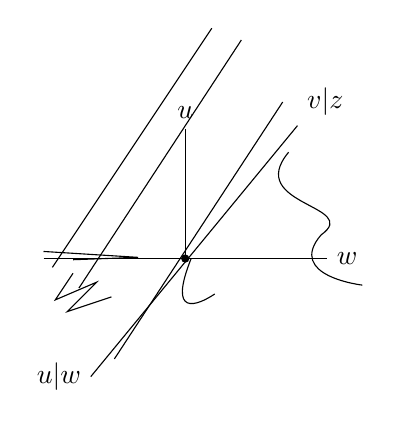
\begin{tikzpicture}[scale=.75]
\draw (-2.4,0)--(2.4,0);
\draw (0,0)--(0,2.2);
\draw (-1.6,-2)--(1.9,2.25);
\fill (0,0) circle (2pt);
\node[above] at (0,2.2) {$\unsure{u}$};
\node[above right] at (1.9,2.25) {$\unsure{v|z}$};
\node[right] at (2.4,0) {$\deleted{\unsure{w}}$};
\node[left] at (-1.6,-2) {$\deleted{\unsure{u|w}}$};
\draw (-2.25,-.15)--(.45,3.9);
\draw (-1.8,-.5)--(.95,3.7);
\draw (-1.2,-1.7)--(1.65,2.65);
\draw (-2.4,.12)--(-.8,.02)--(-1.9,-.02);
\draw (1.75,1.8) .. controls (1.0,.9) and (3,.9) .. (2.3,.4) .. controls (1.7,-.3) and (3,-.45) .. (3,-.45);
\draw (.1,0) .. controls (-.3,-1) and (.2,-.8) .. (.5,-.6);
\draw (-1.9,-.25)--(-2.2,-.7)--(-1.5,-.4)--(-2,-.9)--(-1.25,-.65);
\end{tikzpicture}}
\figure{\begin{tikzpicture}[scale=.85]
\draw (0,0)--(0,1.8) node[above] {$w$};
\draw (0,0)--(1.8,-.25) node[right] {$V$};
\draw (0,0)--(-1.25,-1.65) node[below left] {$\unsure{u|U}$};
\end{tikzpicture}}

\scanpage{72}
% archive sheet number: 71
% The entire opening paragraph is crossed out by large diagonal strokes.
\deleted{Nous allons examiner de plus près le cas où $\alpha,\beta$ sont des racines de polynômes $\frac12$ cyclotomiques $F_p(\alpha)=0,F_{\unsure{q|s}}(\beta)=0$ ($p,q\ge1$, sans exclure les cas $1,2$ qui correspondent \inserted{resp.} aux valeurs $2,-2$ pour $\alpha,\beta\ldots$), \deleted{\unsure{dans}} \inserted{et} le cas \uline{réel} $k=\mathbb{R}$. Si on veut obtenir \unsure{une|un} \deleted{\unsure{homéomorphisme|homéomorphie}} \inserted{\unsure{plongement}} \deleted{\unsure{image}} de la réalisation topologique de la carte combinatoire $C_{p,q}$, il faut prendre (pour $p$ resp. $q$ finis $\ge3$) des valeurs de la $\alpha$ resp. $\beta$ de la forme $\unsure{\zeta|\eta}+\zeta^{-1}$, où $\zeta=\exp 2i\pi/n$ ($n=p$ resp. $q$); d'autre part, $\alpha=-2\inserted{\text{ ou }\beta=-2}$ donne des croisements, donc si $p=\infty$ il faut $\alpha=2$, et $q=\infty$ il faut $\beta=2$.}

\[
\beta=2\qquad\alpha\ne-2
\]
\[
\gamma=2(3+\alpha)+2\alpha=2(2\alpha+3)
\qquad\gamma+2=2(2\alpha+4)=4(\alpha+2)
\]
\[
\begin{aligned}
\delta'&=4-4(\gamma+2)-\gamma^2=-(\gamma^2+4\gamma+4)=-(\gamma+2)^2\\
&=-16(\alpha+2)^2
\end{aligned}
\]
qui n'est nul que si $\alpha=-2$, cas que nous avons exclu\ldots
\[
\begin{aligned}
f_0(x,y,z)&=x^2+y^2+z^2-2(2\alpha+3)yz-2zx-2xy\\
&=\deleted{\unsure{xy|uxy}}(-x+y+z)^2-2(2\alpha+4)yz
\end{aligned}
\]
\[
f_0(x,y,z)=(-x+y+z)^2-4(\alpha+2)yz
\]

\scanpage{74}
\mspage{\unsure{(32)|(22)}}
% archive sheet number: 73
\margin{\unsure{C}}
Calculs en coordonnées universelles

(icosaèdre)

vieille rédaction

\scanpage{75}
% archive sheet number: 74
\figure{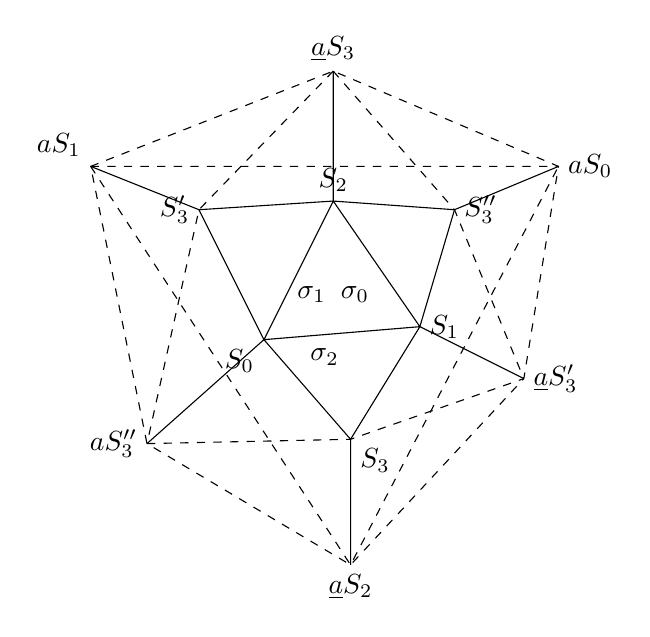
\begin{tikzpicture}[scale=1.1]
\coordinate (s0) at (0,0);\coordinate (s1) at (1.8,.15);\coordinate (s2) at (.8,1.6);\coordinate (s3) at (1,-1.15);
\coordinate (sp) at (-.75,1.5);\coordinate (spp) at (2.2,1.5);
\coordinate (as1) at (-2,2);\coordinate (as0) at (3.4,2);\coordinate (as2) at (1,-2.6);\coordinate (as3) at (.8,3.1);\coordinate (asp) at (3,-.45);\coordinate (aspp) at (-1.35,-1.2);
\draw (s0)--(s1)--(s2)--cycle (s0)--(s3)--(s1) (s0)--(sp)--(s2)--(spp)--(s1);
\draw[dashed] (as1)--(as3)--(as0)--(asp)--(as2)--(aspp)--cycle (as3)--(sp)--(aspp) (as3)--(spp)--(asp) (aspp)--(s3)--(asp);
\draw[dashed,thin] (as1)--(as0) (as1)--(as2)--(as0);
\draw (as1)--(sp) (as0)--(spp) (as3)--(s2) (as2)--(s3) (aspp)--(s0) (asp)--(s1);
\node[below left] at (s0) {$S_0$};\node[right] at (s1) {$S_1$};\node[above] at (s2) {$S_2$};\node[below right] at (s3) {$S_3$};\node[left] at (sp) {$S'_3$};\node[right] at (spp) {$S''_3$};
\node[above left] at (as1) {$aS_1$};\node[right] at (as0) {$aS_0$};\node[below] at (as2) {$\underline aS_2$};\node[above] at (as3) {$\underline aS_3$};\node[right] at (asp) {$\underline aS'_3$};\node[left] at (aspp) {$aS''_3$};
\node at (.55,.52) {$\sigma_1$};\node at (1.05,.52) {$\sigma_0$};\node at (.7,-.2) {$\sigma_2$};
\end{tikzpicture}}
\[
\sigma_0:\quad\begin{aligned}
\inserted{S_0\longrightarrow S_1}\\
\unsure{S_1|S_0}\longleftrightarrow S_0\\
S_2\longmapsto S_2\\S_3\longmapsto S_3
\end{aligned}
\qquad\begin{aligned}
e_1&\longmapsto-e_1\\e_2&\longmapsto-e_1+e_2\\e_3&\longmapsto-e_1+e_3
\end{aligned}
\]
\[
\sigma_0=\begin{pmatrix}-1&-1&-1&1\\0&+1&0&0\\0&0&+1&0\\0&0&0&1\end{pmatrix}
\]
\[
\boxed{\sigma_0(x,y,z)=\deleted{\unsure{\mathrm{id}}}(1-(x+y+z),y,z)}
\]
\figure{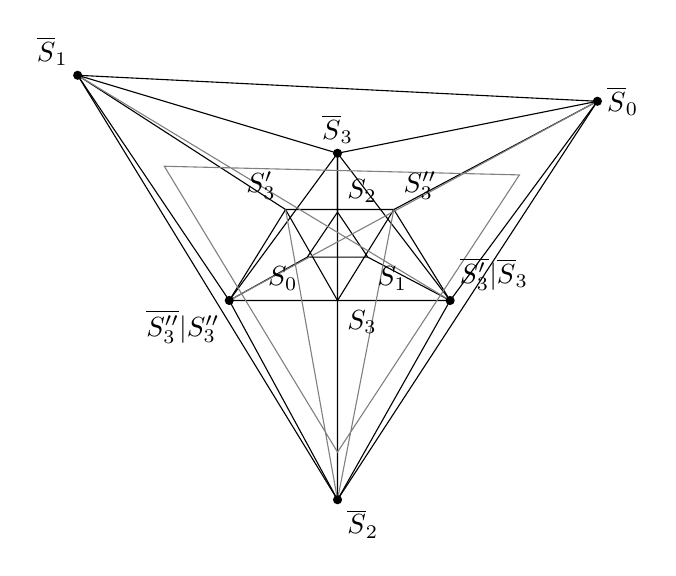
\begin{tikzpicture}[scale=1.1]
\coordinate (A) at (-3,2.6);\coordinate (B) at (3,2.3);\coordinate (C) at (0,-2.3);
\coordinate (t) at (0,1.7);\coordinate (l) at (-1.25,0);\coordinate (r) at (1.3,0);
\coordinate (p) at (-.6,1.05);\coordinate (q) at (.65,1.05);\coordinate (s0) at (-.35,.5);\coordinate (s1) at (.35,.5);\coordinate (s2) at (0,1.02);\coordinate (s3) at (0,0);
\draw (A)--(B)--(C)--cycle (t)--(l)--(r)--cycle;
\draw (A)--(t)--(B) (A)--(p)--(l) (A)--(l) (B)--(q)--(r) (B)--(r) (C)--(l) (C)--(r) (C)--(s3)--(t);
\draw (p)--(q)--(s3)--cycle (s0)--(s1)--(s2)--cycle (l)--(s0) (r)--(s1) (t)--(s2);
\draw[gray,thin] (-2,1.55)--(2.1,1.45)--(0,-1.75)--cycle (A)--(r) (B)--(l) (C)--(p) (C)--(q);
\foreach \P in {A,B,C,t,l,r}{\fill (\P) circle (1.5pt);}
\node[above left] at (A) {$\overline S_1$};\node[right] at (B) {$\overline S_0$};\node[below right] at (C) {$\overline S_2$};\node[above] at (t) {$\overline S_3$};
\node[above left] at (p) {$S'_3$};\node[above right] at (q) {$S''_3$};\node[below left] at (l) {$\unsure{\overline{S''_3}|S''_3}$};\node[above right] at (r) {$\unsure{\overline{S'_3}|\overline S_3}$};
\node[below left] at (s0) {$S_0$};\node[below right] at (s1) {$S_1$};\node[above right] at (s2) {$\unsure{S_2}$};\node[below right] at (s3) {$S_3$};
\end{tikzpicture}}
\[
\sigma_1:\quad\begin{aligned}
S_0&\longmapsto S_0\\S_1&\longmapsto S_2\\S_2&\longmapsto S_1\\S_3&\longmapsto S'_3=S_0+(1+\alpha)(e_2-e_1)+e_3
\end{aligned}
\qquad\begin{aligned}
e_1&\longmapsto e_2\\e_2&\longmapsto e_1\\e_3&\longmapsto(1+\alpha)(e_2-e_1)\inserted{+e_3}\\
&=\alpha'e_1-\alpha'e_2+e_3
\end{aligned}
\]
\[
\sigma_1=\begin{pmatrix}0&1&\alpha'&0\\1&0&-\alpha'&0\\0&0&1&0\\0&0&0&1\end{pmatrix}
\qquad\boxed{\sigma_1(x,y,z)=(y+\alpha'z,x-\alpha'z,z)}
\]
\[
\sigma_2:\quad\begin{aligned}
S_0&\longmapsto S_0\\S_1&\longmapsto S_1\\S_2&\longmapsto S_3\\S_3&\longmapsto S_2
\end{aligned}
\qquad\begin{aligned}
e_1&\longmapsto e_1\\e_2&\longmapsto e_3\\e_3&\longmapsto e_2
\end{aligned}
\]
\[
\sigma_2=\begin{pmatrix}1&0&0&0\\0&0&1&0\\0&1&0&0\\0&0&0&1\end{pmatrix}
\quad\deleted{\unsure{=}}\boxed{\sigma_2(x,y,z)=(x,z,y)}
\]
\[
\left\{\begin{aligned}
H_0:&\quad2x+y+z-1=0\\H_1:&\quad x-y-\alpha'z=0\\H_2:&\quad y-z=0
\end{aligned}\right.
\qquad\left\{\begin{aligned}
\Delta_0:&\quad y=z=0&&\text{i.e. }\Delta_0=\unsure{\underline O_S|\mathcal O_S}\cdot e_1\\
\Delta_1:&\quad z=0,x+y=0&&\text{i.e. }\Delta_{\unsure{1|p}}=\underline O_S(e_1-e_2)\\
\Delta_2:&\quad x=0,y+z=0&&\text{i.e. }\Delta_2=\underline O_S(e_2-e_3)
\end{aligned}\right.
\]
en car. $2$, $H_2\parallel H_0$.
\[
\left\{\begin{aligned}
D_0=H_1\cap H_2:&\quad y=z=\alpha'x\\
D_1=H_2\cap H_0:&\quad y=z=\underbrace{\tfrac12-x}_{\text{(car}\ne2\text{)}}\\
D_2=H_0\cap H_1:&\quad y=\deleted{\unsure{\alpha}}(1-3\alpha)x+\alpha,\quad z=\unsure{-3|3}(1-\alpha)x+(1-\alpha)
\end{aligned}\right.
\]
\[
\begin{aligned}
D_0&=\underline O_S(1,\alpha',\alpha')=\underline O_S(-\alpha,1,1)\\
\underline{\mathrm{hom}\,D_1}:\ (y=z=-x)&=\underline O_S(1,-1,-1)\\
\underline{\mathrm{hom}}(D_2)&=\underline O_S(1,1-3\alpha,\unsure{-3|3}(1-\alpha))
\end{aligned}
\]
\uline{centre}\quad $o=\frac12(\alpha',1-\alpha',1-\alpha')=\deleted{\unsure{\frac12\alpha'}}$

\uline{Antipodisme}
\[
\underline a(x,y,z)=(\alpha'-x,(1-\alpha')-y\unsure{\},},(1-\alpha')-z\unsure{\}})
\]
\[
\tfrac12(-1+\sqrt5\quad\unsure{)|?}=-\unsure{?|2|1}+\unsure{\sqrt5|\sqrt\gamma}
\]

\scanpage{76}
% archive sheet number: 75
\diagram{\(\begin{array}{ll|l}
S_0=(0,0,0)&\underline aS_0=(\alpha',1-\alpha',1-\alpha')&\underline a(x,y,z)=(\alpha'-x,(1-\alpha')-y,(1-\alpha')-z)\\
S_1=(1,0,0)&\underline aS_1=(\alpha'-1,1-\alpha',1-\alpha')&c=\frac12(\alpha',1-\alpha',1-\alpha')\\
S_2=(0,1,0)&\underline aS_2=(\alpha',\unsure{-\alpha'|-\alpha'_2},1-\alpha')&\text{centre}\\
S_3=(0,0,1)&\underline aS_3=(\alpha',1-\alpha',-\alpha')&u=2c=(\alpha',1-\alpha',1-\alpha',2)\\
S'_3=(\alpha',-\alpha',\unsure{2|1})&\underline aS'_3=(0,1\deleted{\unsure{+\alpha'|-\alpha'}},-\alpha')&\\
S''_3=(0,-\alpha',1)&\underline aS''_3=(\alpha',1-2\alpha',-\alpha')&
\end{array}\)}
\[
\begin{aligned}
q_0(x,y,z)&=x^2+y^2+z^2-\alpha yz+\unsure{X|x}(y+z)-(x+y+z)\\
\bigl[&=(\text{en car. }2)\quad\alpha'\bigl[(x-\alpha y)^2+\alpha'(x-\alpha y)(x-\alpha z)+(x-\alpha z)^2\bigr]\\
&\hspace{7em}-(x+y+z)\bigr]
\end{aligned}
\]
Si $e$ est un vecteur arête (tel que $s_1-s_0=e_1$),
\[
f\quad\text{---}\quad\text{coarête}\quad(\text{tel que }s_3-s_2=e_3-e_2)
\]
\[
\left\{\begin{aligned}
q(e)&=1\quad\text{(c'est la normalisation de }q\text{ !)}\\
q(f)&=\alpha+2\\
q(f)/q(e)&=\alpha+2=(\alpha+1)^2=\alpha'^2
\end{aligned}\right.
\]
En coordonnées distinguées, si $(\pm x,\pm y,0),(\deleted{\unsure{+}}\pm y,0,\pm x),(0,\pm x,\pm y)$ sont les $12$ sommets de l'icosaèdre, on aura (si $(x,y,0)$ et $(-x,y,\unsure{0})$ sont les sommets d'une arête, donc $(x,y,0)$ et $(x,-y,0)$ ceux d'une coarête)
\figure{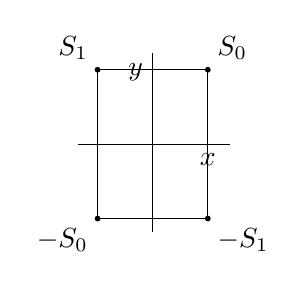
\begin{tikzpicture}[scale=.7]
\draw (-1,-1.35) rectangle (1,1.35);
\draw (0,-1.6)--(0,1.65) (-1.35,0)--(1.4,0);
\fill (-1,1.35) circle (1.5pt);\fill (1,1.35) circle (1.5pt);\fill (-1,-1.35) circle (1.5pt);\fill (1,-1.35) circle (1.5pt);
\node[above left] at (-1,1.35) {$S_1$};\node[above right] at (1,1.35) {$S_0$};\node[below left] at (-1,-1.35) {$-S_0$};\node[below right] at (1,-1.35) {$-S_1$};\node[left] at (0,1.3) {$y$};\node[below] at (1,0) {$x$};
\end{tikzpicture}}
\[
\deleted{\unsure{\frac{4y^2}{4x^2}=\lambda\left(\frac yx\right)^2}}\deleted{\unsure{\alpha}}\frac{q(f)}{q(e)}=\frac{4y^2}{4x^2}=\left(\frac yx\right)^2=\alpha'^2\quad\text{donc}\quad\frac yx=\pm\alpha'
\]
(dans le cas réel, \unsure{l'icosaèdre|d'icosaèdre} convexe, $\alpha=\frac12(-1+\sqrt5)$, $\alpha'=\frac12(-1-\sqrt5)$, \deleted{\unsure{et}} et si on prend $x,y>0$, on trouve $y/x=-\alpha'=\frac12(1+\sqrt5)$)
\[
\delta'(q_0)=1\qquad\text{Matrice }\unsure{\varphi|\phi}_{q_0}=\begin{pmatrix}2&1&1\\1&2&-\alpha\\1&-\alpha&\deleted{\unsure{0}}2\end{pmatrix}
\]
Matrice non singulière sauf en car. $2$, où le noyau de $\varphi_{q_0}$ est engendré par le vecteur $u=(\alpha',1-\alpha',1-\alpha')=(\alpha',\alpha,\alpha)=(1+\alpha,\alpha,\alpha)$ NB $q_0(u)=\alpha'\ne0$, ce qui exprime la \unsure{non-singularité|nonsingularité} de $q_0$ en car. $2$)

\scanpage{77}
% archive sheet number: 76
\uline{vecteurs remarquables} \inserted{\uline{de directions remarquables}} (cas car. $\ne2$)

On suppose $2$ inversible : son centre $o$ identifiant $E$ et l'espace des translations $V$. Utilisant la forme quadratique, on identifie aussi $V$ et $\check V$ -- donc $\check{\mathbb P}(V)$ (directions de droites de $E$) et $\mathbb P(V)$ (directions de plans de $E$).

\margin{$S$}
$12$ vecteurs ``\inserted{doubles} sommets'' $\boxed{S_i-\underline aS_i}$

\margin{$\Delta$}
$30$ vecteurs \deleted{\unsure{arêtes}} \inserted{arêtes} $S_i-S_j$ $(\{i,j\}\in A)$ se groupent en $15$ paires de vecteurs opp.
\margin{\uline{NB} chaque arête détermine deux vect, mais deux arêtes opposées déterminent les mêmes deux}

\margin{$\Delta'$}
$30$ vecteurs coarêtes $S_i-S_j$ $(\{i,j\}\in A')$ ce sont les $\unsure{\pm}\alpha'u$ $(u\in\Delta')$
\deleted{\unsure{les mêmes en car.} $\unsure{\Delta}$ \unsure{deux}}
\[
\boxed{\Delta'=\alpha'\Delta,\quad\Delta=\alpha\Delta'}
\]
\diagram{\begin{tikzcd}[ampersand replacement=\&]
{}\arrow[r]\&{}\\
{}\arrow[u]\arrow[r]\&{}\arrow[u]
\end{tikzcd}}
\deleted{les vecteurs}

\margin{$\left[\begin{matrix}\mathcal A\\\mathcal A'\end{matrix}\right.$}
Les \inserted{\deleted{\unsure{doubles}} $30$} milieux d'arête $\deleted{\tfrac12}(S_i+S_j-2c)$ $(\{i,j\}\in A)$

\unsure{---} \inserted{$30$} de coarête $\frac12(S_i+S_j)$ $(\{i,j\}\in A')$
\[
\begin{aligned}
\Delta&=\deleted{\unsure{\xi}}2\mathcal A'&\left\{\begin{aligned}\mathcal A&=\alpha'\mathcal A'\\\mathcal A'&=\alpha\mathcal A\end{aligned}\right.\\
\Delta'&=\deleted{\unsure{\xi}}\unsure{2}\mathcal A
\end{aligned}
\]
i.e. $\Delta$ est aussi formé des $S_i+S_j$ $(\{i,j\}\in A')$
\[
\Delta'\quad\text{---}\qquad(\{i,j\}\in A)
\]

\margin{$\Phi$}
Les \inserted{$20$ triples (\unsure{ou hexuples|ou hexagones}\ldots)} barycentres des faces $\deleted{\tfrac13}(S_i\unsure{+|-}S_j\unsure{-|+}S_h\unsure{+|-}3c$ $(\{i,j,h\}\in F)$

\margin{$\Phi'$}
Les \inserted{$20$ triples} barycentres des cofaces $(\{i,j,h\}\in F')$
\margin{$\unsure{26\text{ bis}|2\text{ triples}|2\text{ trpls}}$}
\[
\Phi'=\lambda\Phi,\quad\Phi=\lambda'\Phi'\qquad(\lambda\lambda'=\mathrm{Norm}(\lambda)=\deleted{\unsure{-}}1)\qquad\lambda=2\alpha-1
\]
\deleted{\unsure{en 20}}
($\Phi$ et $\Phi'$ sont homothétiquement les sommets des Dodécaèdres inscrits dans $\Pi$ et dans le contreicosaèdre associé $\Pi'$)

\margin{$\Psi$}
Les $20$ sommets \inserted{\uline{multipliés par $10$}} des dodécaèdres circonscrits \inserted{à $\Pi$} : intersections des plans des faces adjacentes à une face

\margin{$\Psi'$}
\unsure{it.|idem} pour $\Pi'$
\[
\Psi'=\unsure{\nu|\mu}\Psi,\quad\Psi=\nu'\Psi'\qquad\deleted{\mu\mu'=\mathrm{Norm}(\mu)=1}\quad\nu=-\lambda
\]
\[
\boxed{\Psi=\mu\Phi,\quad\Psi'=\mu'\Phi'}
\qquad\begin{aligned}
\mu&=1+2\alpha=-(1+2\alpha')\\
(\mu\mu'&=-5),\quad\mu^2=5\text{ i.e. }\mu=\sqrt5
\end{aligned}
\]
\inserted{$\mu'=-\mu$}

\margin{$\Sigma$}
Les $12$ \inserted{\unsure{quintuples|quadruples}} barycentres des pentagones inscrits aux sommets
\[
2(S_1+S_2+S_3+S_4+S_0)-2c
\]
\[
\begin{aligned}
\Sigma&=\rho S=\rho'S\qquad\rho'=-\rho\quad\text{i.e. }\deleted{\rho=\rho+\rho'c}\inserted{\mathrm{Tr}\rho=0}\\
\rho&=\mu=1+2\alpha\ldots
\end{aligned}
\]

\scanpage{78}
% archive sheet number: 77
% Typescript upside down in scan; transcribed in its upright reading order.
\mspage{- 2 -}

- il émet un avis sur le profil des postes disponibles.

- il apporte son concours à l'orientation des chercheurs en difficulté.

II.- \uline{COMPOSITION DU CONSEIL SCIENTIFIQUE}.

Sous la présidence du Président de l'Université, le conseil comprend :
\begin{itemize}[label={},leftmargin=3em]
\item n membres ès qualité
\item 2n membres élus
\item des personnalités extérieures (dans la limite de 10 \% des membres ès qualité et élus).
\end{itemize}

- \uline{Les membres ès qualité} :

Ils appartiennent à l'U.S.T.L. et sont au nombre de n. Ils comprennent les personnalités nommées ou élues dans les charges nationales ou locales suivantes :
\begin{itemize}[label=$\cdot$]
\item les membres de l'Académie et correspondants,
\item les directeurs des formations propres et associées du C.N.R.S., si ces formations comportent au moins dix docteurs d'Etat,
\item les membres du comité national de la recherche scientifique, des comités de disciplines des grands organismes de recherche (enveloppe recherche) appartenant au collège électoral.
\item le président du conseil scientifique de l'Ecole nationale supérieure d'ingénieurs de chimie de Montpellier.
\end{itemize}

La liste des membres ès qualité est établie par le Président de l'Université un mois au moins avant la date fixée pour l'élection des membres élus du conseil scientifique.

- \uline{Les membres élus}.

Ils sont au nombre de 2n. Leur élection a lieu conformément aux dispositions des articles 9, 11 et 12 des présents statuts.

\begin{enumerate}[label=a)-]
\item \uline{Collège électoral} : collège unique composé des membres de l'U.S.T.L. exerçant les fonctions de professeurs, directeur de recherche, maître de conférences, maître de recherche, maître-assistant, chargé de recherche et chercheurs de niveau équivalent inscrits, soit sur la liste d'aptitude aux fonctions de maître de conférences, soit sur celle de maître de recherche.
\end{enumerate}

Tous les électeurs sont éligibles, à l'exception des membres ès qualité.

\scanpage{79}
% archive sheet number: 78
Directions remarquables
\[
\begin{aligned}
\unsure{6}&\quad\text{directions de \unsure{sommet|sommets}}\\
15&\quad\text{--- d'arêtes}\\
\underline{10}&\quad\text{directions de faces}\\
31&=5^2+5+1\quad\text{nb de pts du plan projectif sur }\mathbb F_5
\end{aligned}
\]
Les 6 directions de \unsure{sommet|sommets} correspondent à la \unsure{conique}. Les \inserted{15} directions d'\deleted{\unsure{faces}}\inserted{arêtes} correspondent aux sécantes découpant un diviseur \deleted{$\unsure{\to}$}\inserted{\unsure{décomposé}}$/\mathbb F_5$ ; les \inserted{10} directions de faces correspondent aux diviseurs \unsure{connexes} $/\mathbb F_5$.

vecteurs remarquables en \uline{car. 5}
\[
1+12+60+40=11\deleted{\unsure{2}}3
\qquad
125=\underset{\infty}{1}+\underbrace{24}_{\substack{\text{pts sur}\\\text{la conique}\\=2\times12\\\text{(deux ico.)}}}+60+40
\]
\unsure{des|les} \deleted{\unsure{quinze}}\inserted{25} \unsure{droites|doubles} non isotropes

\deleted{\unsure{20}\ \unsure{points}}\inserted{15}\ \deleted{\unsure{plans}} associés aux \deleted{\unsure{arêtes}}\inserted{arêtes}\ \deleted{\unsure{les points}}\ \deleted{\unsure{dist.|distincts}}.

\deleted{\unsure{distingués}}

20 aux faces --- elles sont \inserted{\unsure{donc}}

\figure{%
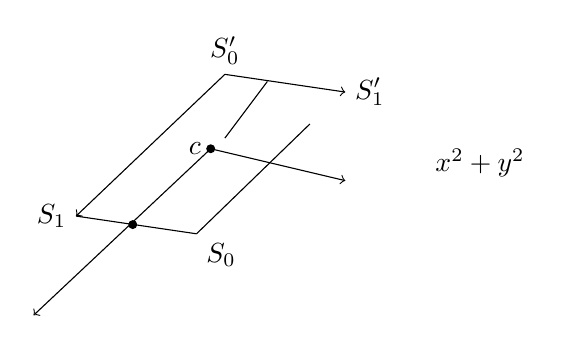
\begin{tikzpicture}[scale=.9]
\coordinate (s1) at (0,0);\coordinate(s0) at (1.7,-.25);
\coordinate(sp0) at (2.1,2);\coordinate(sp1) at (3.8,1.75);
\draw[->] (sp0)--(s1);\draw (s1)--(s0);\draw[->] (sp0)--(sp1);
\draw (2.7,1.9)--(2.1,1.1);\draw (s0)--(3.3,1.3);
\draw[->] (1.9,.95)--(-.6,-1.4);\draw[->] (1.9,.95)--(3.8,.5);
\fill (.8,-.12) circle(1.8pt);\fill(1.9,.95) circle(1.8pt);
\node[left] at(s1){$S_1$};\node[below right] at(s0){$S_0$};
\node[above] at(sp0){$S'_0$};\node[right] at(sp1){$S'_1$};
\node[left] at(1.9,.95){$c$};
\node at(5.7,.75){$\deleted{x^2+y^2}$};
\end{tikzpicture}}

% archive/scan mark: isolated right-angle registration-like mark near lower edge

\scanpage{80}
% archive sheet number: 79
% archive/scan mark: right-angle registration-like mark at edge (upright upper left)
% Typescript upside down in scan; transcribed in its upright reading order.
\uline{STATUTS de l'UNIVERSITE DES SCIENCES ET TECHNIQUES DU LANGUEDOC}

\uline{Article 20} (Nouvelle rédaction approuvée par le conseil de l'Université le 29 juin 1977).

\begin{center}
--

\fbox{CONSEIL SCIENTIFIQUE}
\end{center}

I.- \uline{MISSION}.

Conformément aux dispositions de l'article 13 de la loi d'orientation de l'enseignement supérieur, un conseil scientifique détermine les programmes de recherche et répartit les crédits correspondants. Pour cela :
\begin{itemize}[label=-]
\item il garantit le libre arbitre des universitaires dans le choix des axes de recherche,
\item il favorise la participation des équipes de l'Université à des travaux s'insérant dans les axes des programmes de recherche internationaux, nationaux et régionaux.
\item il établit les bilans et propose les choix en ce qui concerne la politique de recherche scientifique, compte tenu du potentiel de recherche des laboratoires, des axes de recherche de l'Université et de la politique définie par les organismes internationaux, nationaux et régionaux.
\item il répartit les crédits de fonctionnement de recherche non affectés de la façon suivante :
\begin{itemize}[label=$\cdot$]
\item une partie attribuée en tenant compte du nombre et de l'encadrement des laboratoires;
\item une partie attribuée sur programme. La partie attribuée sur programme est utilisée notamment pour :
\begin{itemize}[label=-]
\item aider les jeunes équipes pour leur permettre d'atteindre le seuil de prise en charge par les organismes nationaux;
\item assurer les équipements d'intérêt collectif (laboratoire ou service commun);
\item apporter son soutien aux formations ayant un programme reconnu sur le plan national, ou dont il reconnaîtra l'intérêt;
\item mettre en place des opérations susceptibles d'être soutenues et relayées par les organismes nationaux et régionaux (C.N.R.S., D.G.R.S.T., etc.).
\end{itemize}
\end{itemize}
\end{itemize}

\scanpage{81}
% archive sheet number: 80
\[
y=z\qquad x=(1+\alpha')y=-\alpha y\qquad y=\alpha'x
\]
\[
\begin{aligned}
\underline{(-\alpha y,y,y)}&\quad\text{ou}\quad(x,\alpha'x,\alpha'x)\\
(-\alpha,1,1)&\qquad(1,\alpha',\alpha')\\
-\alpha&=\alpha'(1-\alpha')=\alpha'-\alpha'^2\\
\alpha'&\overset{?}{=}-\alpha(1-\alpha')=-\alpha-1\quad\text{OK}
\end{aligned}
\]
\margin{$\begin{aligned}1-(2-\alpha)\\\alpha-1\\\alpha=\tfrac12\\\tfrac14+\tfrac12-1=0\\1+2-4=0\\-1=0\\\unsure{\infty}\end{aligned}$}
\[
e_1\ \unsure{\text{non.}}\qquad
\left\{\begin{aligned}
\bar S_0&=(-\alpha,1,1)\\
\bar S_1&=\sigma_0\bar S_0=(\alpha-1,1,1)\\
\deleted{\unsure{e}}\quad\bar S_{\unsure{1|2}}-\bar S_0&=(\underline{2\alpha-1},0,0)
\end{aligned}\right.
\]
\[
\unsure{\alpha'^2|\alpha^2}=1-\alpha'\qquad \alpha+\alpha'=-1
\]
\margin{$\begin{aligned}\deleted{2\alpha}\ 2\\2\alpha-1=2\alpha+2-3\\\deleted{\unsure{\alpha-2}}
\end{aligned}$}
\[
\unsure{\underline{O}_S|\mathcal O_S}\quad(-\alpha,1,1)
\]
\figure{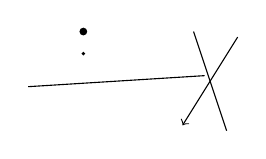
\begin{tikzpicture}[scale=.7]
\fill(1,1)circle(2pt);\fill(1,.6)circle(1pt);
\draw(0,0)--(3.2,.2);\draw(3,1)--(3.6,-.8);\draw[->](3.8,.9)--(2.8,-.7);
\end{tikzpicture}}
\[
\begin{aligned}y+z+1&=0\\x+y+\alpha z&=0\\y&\underline{=z}\end{aligned}
\qquad f(0)=f(\sigma_1\sigma_2)=0
\]
\[
\begin{aligned}f(\sigma_0^2)&=f(\sigma_0)+\sigma_0f(\sigma_0)=0\\
e+\sigma_0e&=0\\\boxed{\sigma_0e=-e}
\end{aligned}
\]
\diagram{\begin{tikzcd}[ampersand replacement=\&]
\&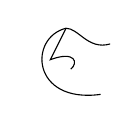
\begin{tikzpicture}[scale=.4]
\draw (1.4,0) .. controls (-.8,-.3) and (-.9,1.8) .. (.3,2.1) .. controls (.7,2.1) and (1,1.4) .. (1.7,1.6);
\draw (.3,2.1)--(-.2,1.1) .. controls (.6,1.4) and (.7,1) .. (.45,.8);
\end{tikzpicture}\\
\unsure{\Gamma|\mathscr G}\arrow[r]\&SO^{\unsure{\uparrow|+}}(q)
\end{tikzcd}}
$+\ 1$-cocycle
\[
\left\{\begin{aligned}
\Gamma&\overset{\unsure{f}}{\longrightarrow} E\\
f(gg')&=f(g)+gf(g')
\end{aligned}\right.
\]
Il suffit de donner
\[
f(\sigma_1)=f(\sigma_2)=0\qquad \unsure{C|f}(\sigma_0)=e\deleted{\unsure{q}}
\qquad\boxed{q_0(e)=1}
\]
\diagram{\begin{tikzcd}[ampersand replacement=\&,column sep=small,row sep=small]
\&S_2\&\\S_0\arrow[rr,no head]\&\&S_1
\end{tikzcd}}
\[
\begin{aligned}S_2-S_0\\=\\e_2-e_3\\(0,1,-1)\end{aligned}
\]
\[
\sigma_0\sigma_2\sigma_0\sigma_2
\]
\[
\begin{aligned}f(\sigma_0\sigma_2)&=\deleted{\unsure{e+}}e\\
f&\qquad e+\sigma_0\sigma_2e=0\\
\deleted{\boxed{\sigma_0\sigma_2e=\deleted{\unsure{\sigma_2}}-e}}\\
&=\sigma_0e\\
\sigma_0(\sigma_2e-e)&=0
\end{aligned}
\]
\[
\sigma_0\sigma_1=u\qquad
\begin{aligned}
f(u)&=e\\f(u^2)&=e+ue\\f(u^3)&=e+ue+
\end{aligned}
\]
\[
\left\{\begin{aligned}\underline{e_1\wedge e_2\wedge e_3}\\q\end{aligned}\right.
\qquad
\begin{aligned}
f(u^3)&=f(uu^2)=\\&e+u(e+ue)\\&=e+ue+u^2e=0
\end{aligned}
\]
\[
1+1+\alpha=2+\alpha=\deleted{\unsure{\alpha}}1-\alpha'=\boxed{\alpha'^2}
\]
\[
\boxed{\left\{\begin{aligned}\sigma_0e&=-e\\\sigma_2e&=e\end{aligned}\right.}
\quad\begin{aligned}\Longleftrightarrow(1+\sigma_0)e&=0\\\Longleftrightarrow(1+\sigma_0\sigma_2)e&=0\end{aligned}
\qquad\boxed{(1+u+u^2)e=0}
\]
\[
\deleted{\unsure{(1+u+u^2)e}}\qquad
\deleted{(1+u+u^2+u^3+u^4)e=0}\quad\unsure{\zeta|\}}
\]

\scanpage{82}
% archive sheet number: 81
% letterhead
\begin{center}
THE UNIVERSITY OF ROCHESTER\\
\textsc{Department of Mathematics}\\
\textsc{Mathematical Sciences Building}\\
ROCHESTER, NEW YORK 14627
\end{center}
Charles E. Watts, \textit{Chairman}\hfill Phone 716-275-4413\\

\begin{flushright}
September 21, 1977\\
\end{flushright}

Professor A. Grothendieck\\
Institut des Hautes Études Scientifiques\\
91440 Bures-sur-Yvette\\
France\\

Dear Professor Grothendieck:\\

We are considering the reappointment of Professor Saul Lubkin and should very much appreciate your advice in the matter. Lubkin came to Rochester in 1974 on a one-year visiting professorship which was renewed the following year. In 1976 he began a two-year regular (tenure-track) appointment, and he must be notified formally by January 31, 1978 whether or not this appointment will be continued. He can legally be reappointed once more, for a period of up to five years. The question of tenure is administratively separate at Rochester in this case and need not be decided at this point, although we may well consider the question. At any rate, we need at this time an evaluation of his scientific and professional accomplishment and potential, and we hope that you can help us.

We are sending under separate cover all available reprints and preprints; these need not be returned. We enclose a post card which we would like you to return as soon as possible. Finally, we should like to express our gratitude for any assistance you can render in this difficult but essential professional task, and apologize for the shortness of time available.

\begin{flushright}
Sincerely,\\
\handwritten{Charles E. Watts}\\
Charles E. Watts\\
\end{flushright}

CEW:rec\\

Enclosure
